\section{Scaling performance of $4096\times512\times512$ problem}
The last benchmark deal with very large problems. Like for the previous large problem, the dimensions are so huge to require the adoption of multiple processors to run, otherwise we will face an out of memory error.
On a Intel Xeon Phi~\cite{intel:xeonphi} the minimum requirements are to employ at least 2 processors and use 32 cores, or less, per processor.
\par
As the previous problem have highlighted, the less cores are used and the better results are scored, so our impossibility to go further than 32 cores per processor, as pointed some rows before, would not be a big deal. We may suppose that the poorest results will be achieved by 32 cores runs, instead of the 64 ones. \\
\par

\begin{figure}
\begin{center}
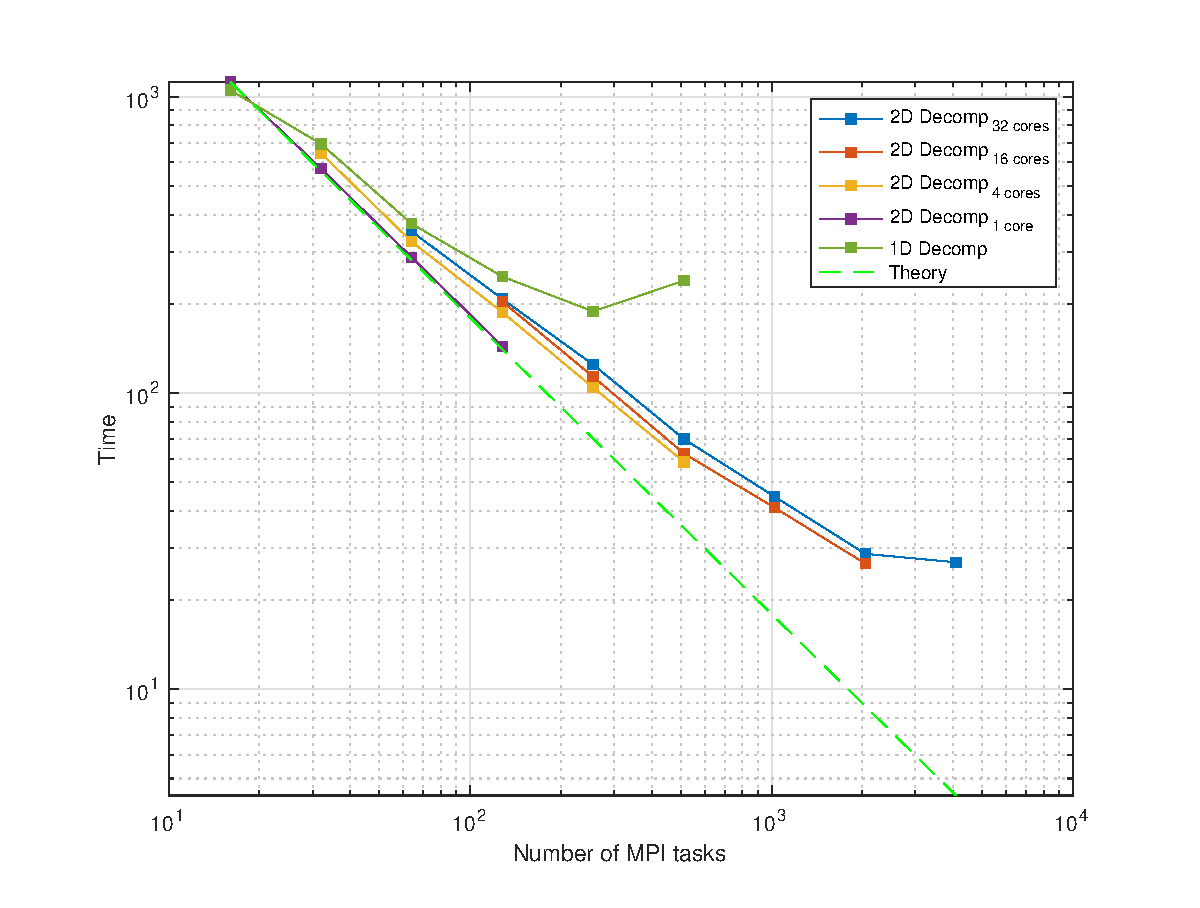
\includegraphics[scale=0.55]{grafici/20481}
\caption{Time scaling comparison for $4096\times 512\times 512$ simulation}
\label{20481}
\end{center} 
\end{figure}

Let us start showing figure~\ref{20481} in which is reported the time scaling of our code.\par
As could be seen, the 2D decomposition using single core achieved the lowest timing execution.
It is interesting to denote how this combination fits the theoretical behavior perfectly.\par
All other 2D decomposed combinations exploit a worse behavior with respect to the single core run, with a marked trend, where the increase in cores per processor number leads to poorer performances. \par 
Such behavior is aligned with our predictions.\\

\begin{figure}
\begin{center}
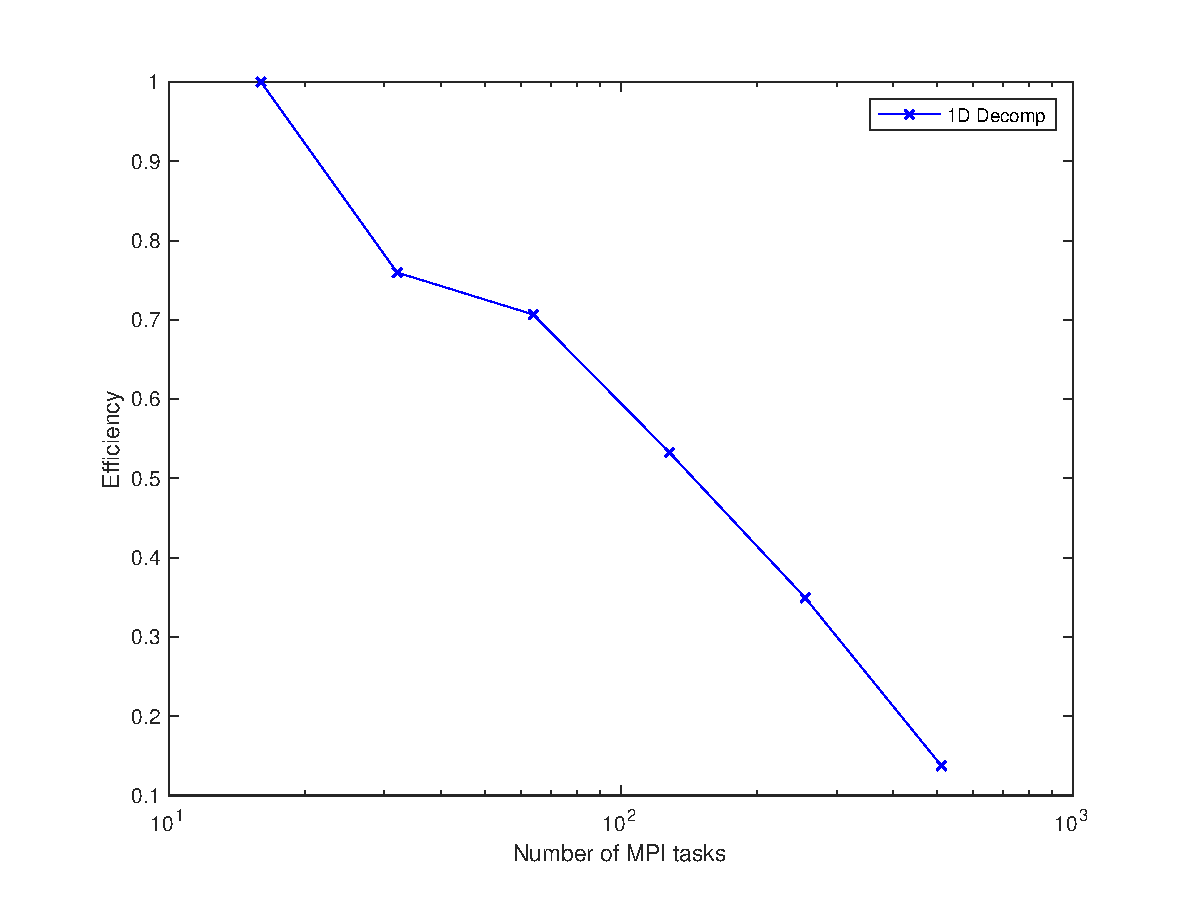
\includegraphics[scale=0.55]{grafici/20483}
\caption{Efficiency factor of $4096\times512 \times512$ simulation using 1D decomposition}
\label{20483}
\end{center}
\end{figure}

\begin{table}
\caption{Data from $4096\times 512\times 512$ simulation, 1D decomposition}
\begin{center}
\begin{tabular}{c c c c}
\toprule
\textbf{\#Processes} & \textbf{Time [s]} & \textbf{Speedup} & \textbf{Efficiency [\%]}\\
\midrule
16 & 1052.9 & 16 & 100\\
32 & 693 & 24.31 & 76\\
64 & 372.5 & 45.23 & 71\\
128 & 247 & 68.2 & 53\\
256 & 188.5 & 89.37 & 35\\
512 & 239.5 & 70.34 & 14\\
\bottomrule
\end{tabular}
\end{center}
\label{2048:data:1}
\end{table}

\par
For what concern about the 1D decomposed algorithm, which, since the code structure is slightly different, can run also on 64 cores per processor, it achieve the worst performances among all possible solutions, highlighting once again the benefits of using a pencil decomposed approach. \par
The speedups achieved by this kind of domain decomposition can be seen in table~\ref{2048:data:1} while the efficiency graph, which shows a poor behavior, can be seen in figure~\ref{20483}. \\
\par



Far more interesting, are the data in table~\ref{2048:data:2}, which report the speedups, efficiency and timing achieved by the algorithm with 2D decomposition. The data, and the graphical counterpart which can be seen in figure~\ref{20482} and~\ref{20484}, report a very high efficiency using single core, while, although smaller, a still high efficiency is preserved by using 4 cores per processor.\\
\par
\begin{figure}
\begin{center}
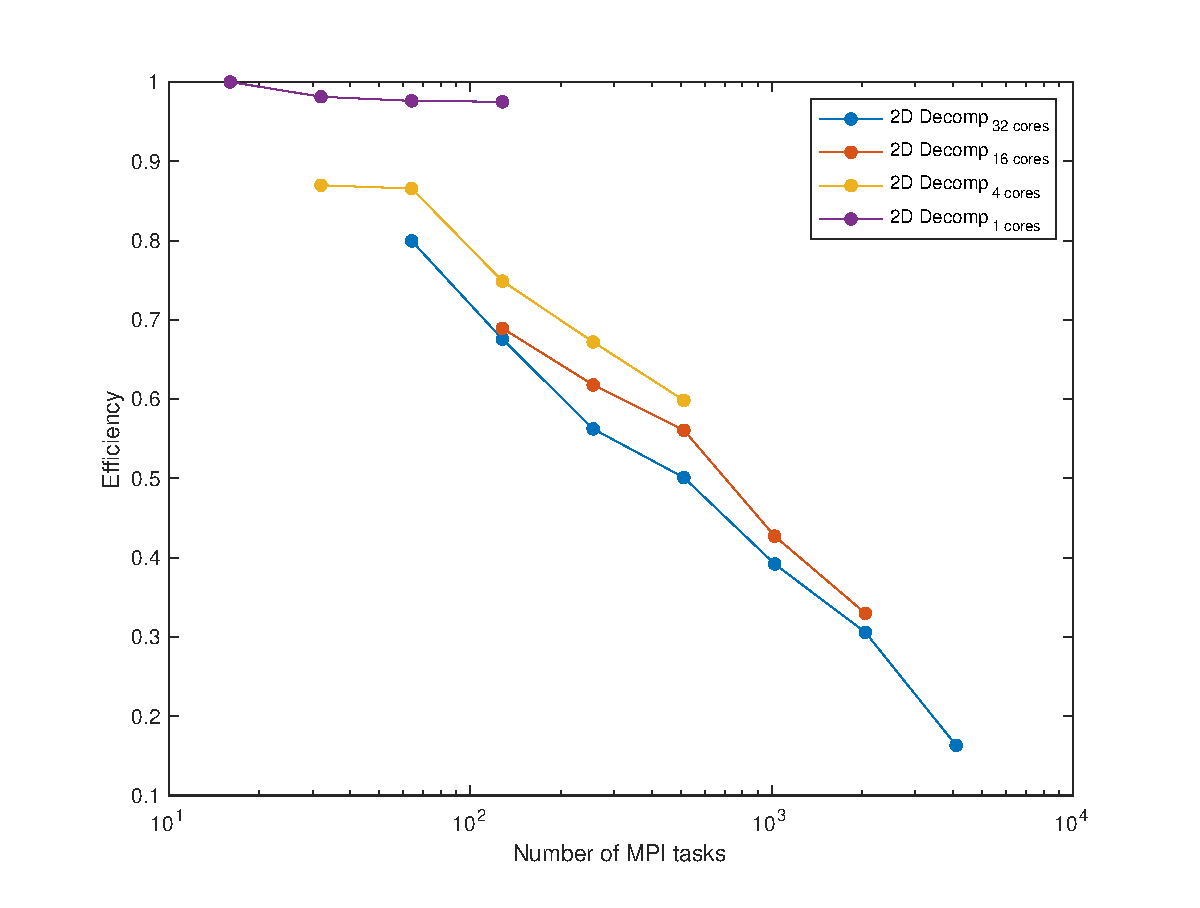
\includegraphics[scale=0.55]{grafici/20484}
\caption{Efficiency factor of $4096\times512 \times512$ simulation using 2D decomposition}
\label{20484}
\end{center}
\end{figure}
Increasing the counter of threads per processor leads to constant losses, as expectable. However, such losses between adjacent stations are lower than the ones of the previous simulations, furthermore we can see wider gaps among the efficiency curves, symptom that there is wider room for improvements.\par
Moreover, at very high number of cores, the efficiency curves slope is minor than before, preserving efficiency and allowing us to perform faster computations with greater speedups.\\
\par
To talk about speedups is useful to introduce figure~\ref{20482}, in which these are reported.\par
The graph, on page~\pageref{20482}, shows the results achieved by the 1D and 2D domain decomposed algorithm, with emphasis on the effects of the variation of cores per processor quantity, for the 2D algorithm only.\par
As has been done in the previous section, the high efficiency shown by the single core run, combined with the physical impossibility to use less cores due to memory limitations, has lead us to made the assumption of speedup equal to 16 for a 16 parallel processes run in a single core environment. All other efficiencies and speedups have been derived using such data as reference.\\
\par

\begin{table}
\caption{Data from $4096\times 512\times 512$ simulation, 2D decomposition}
\begin{center}
\begin{tabular}{c c c c c}
\toprule
\textbf{\#Processes} & \textbf{Time [s]} & \textbf{Speedup} & \textbf{Efficiency [\%]} & \textbf{cores}\\
\midrule
16 & 1121.5 & 16 & 100 & 1\\
\hline
\multirow{2}{*}{32} & 571.4 & 31.4 & 98 & 1\\
& 644.8 & 27.83 & 87 & 4\\
\hline
\multirow{3}{*}{64} & 287.2 & 62.47 & 98 & 1\\
& 323.9 & 55.39 & 87 & 4\\
& 350.7 & 51.17 & 80 & 16\\
\hline
\multirow{4}{*}{128} & 143.8 & 124.8 & 98 & 1\\
& 187.2 & 95.85 & 75 & 4\\
& 203.4 & 88.23 & 69 & 16\\
& 207.5 & 86.47 & 68 & 32\\
\hline
\multirow{3}{*}{256} & 104.3 & 172 & 67 & 4\\
& 113.4 & 158.2 & 62 & 16\\
& 124.6 & 144 & 56 & 32\\
\hline
\multirow{3}{*}{512} & 58.6 & 306.4 & 60 & 4\\
& 62.5 & 287.1 & 56 & 16\\
& 70 & 256.5 & 50 & 32\\
\hline
\multirow{2}{*}{1024} & 41 & 437.5 & 43 & 16\\
& 44.7 & 401.4 & 39 & 32\\
\multirow{2}{*}{2048} & 26.6 & 675.5 & 33 & 16\\
& 28.7 & 626.3 & 31 & 32\\
\hline
4096 & 26.8 & 668.8 & 16 & 32\\
\bottomrule
\end{tabular}
\end{center}
\label{2048:data:2}
\end{table}

As can be seen in table~\ref{2048:data:2} the best result is achieved using 16 cores per processor and 2048 parallel processes. Unfortunately, due to some policy limitations, we can not push forward our resources request, although the graph clearly shows margins of improvements for such configuration.\\
\par
Differently from all the previous simulations, the processor grid for the pencil decomposition results balanced when the streamwise stencil has half the modes with respect to the other direction. Such configuration has been suggested by benchmarks.
\par
In conclusion we may say that, although the modes distribution results unbalanced in this simulation, the speedup trend still remain aligned with the ones exhibited in the other simulations.
\begin{figure}
\begin{center}
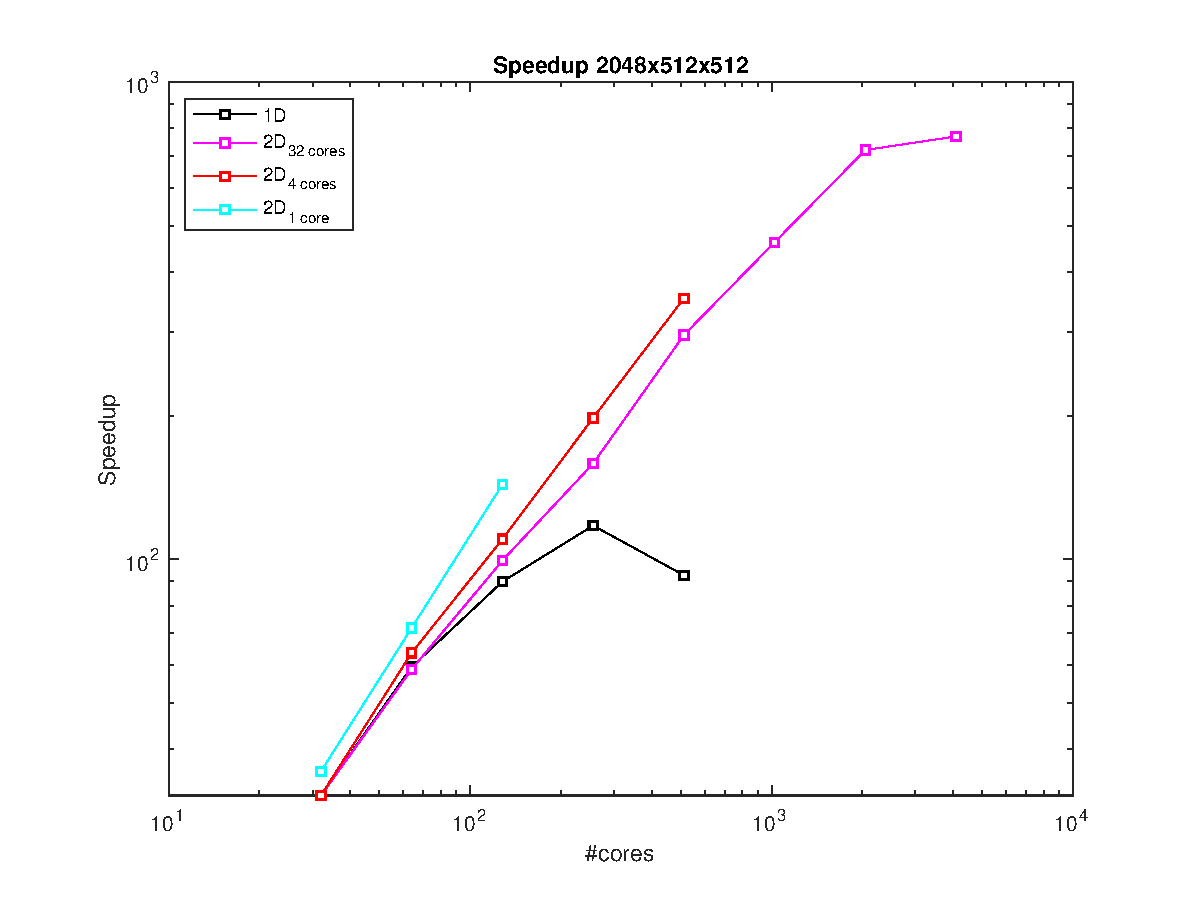
\includegraphics[scale=0.55]{grafici/20482}
\caption{Speedup factor of $4096\times512 \times512$ simulation}
\label{20482}
\end{center}
\end{figure}


\section{Further tests}

\subsection{Intel compiled code performances}
Not happy of the previous results, we decided to move from GCC to Intel proprietary compiler, as advised also by the Cineca authorities.
The Intel C++ Compiler 18 is designed to take care of the MIC architecture, using dedicated flags during the compilation process.\par
Using 
\begin{lstlisting}
-AVX512 -parallel
\end{lstlisting}
flags is possible to instruct the compiler to generate vectorized code autonomously. Although there are no guarantees that all loops will be vectorized, leading this solution to be less efficient than an OpenMP implementation, the usage of these flags speeded up our code roughly of a factor two, providing also doubled efficiency with respect to the previous GCC solution, as can be seen comparing figure~\ref{intel:speedup} with~\ref{1287} and figure~\ref{intel:efficiency} with~\ref{1289}.\\~\\

\begin{figure}
\begin{center}
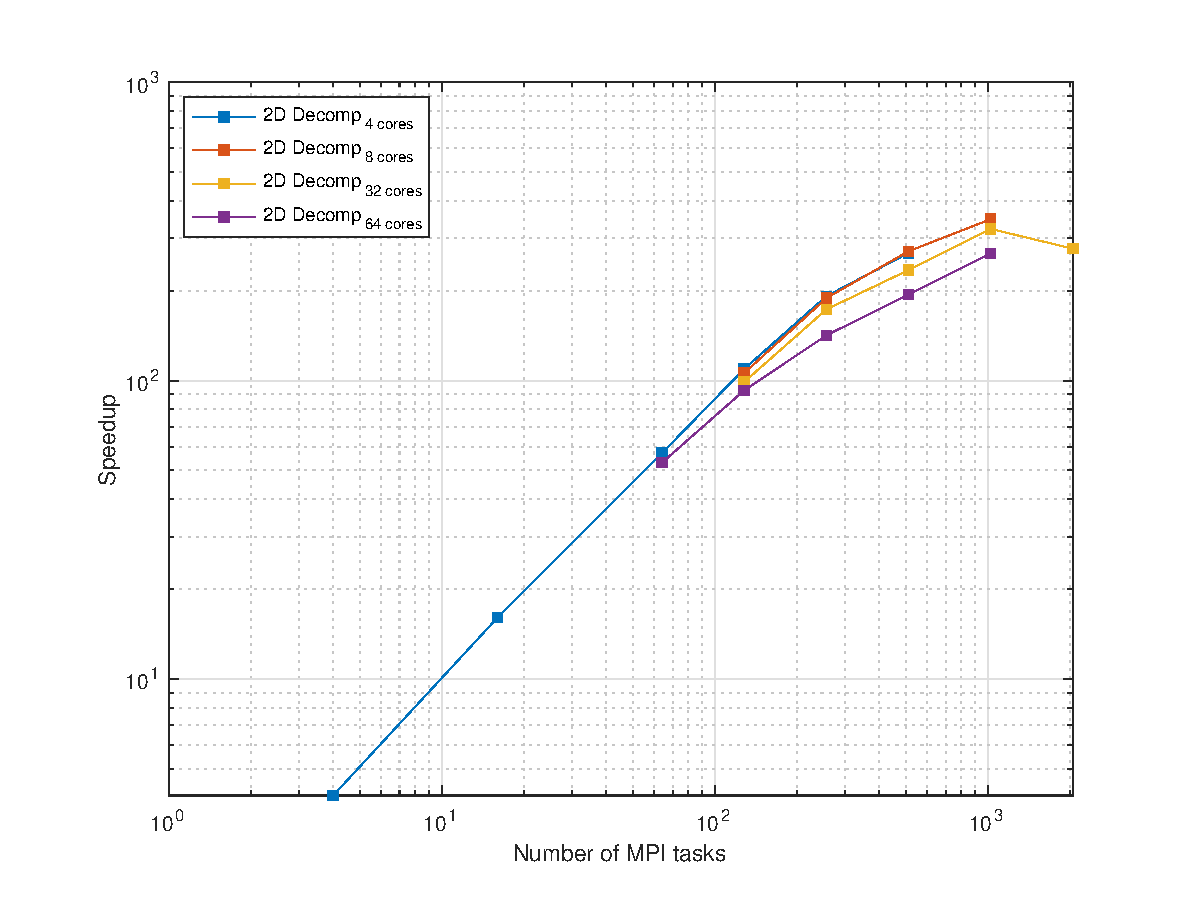
\includegraphics[scale=0.55]{grafici/intel_speedup}
\caption{Speedup using 2D decomposition for $256\times 256\times 512$  simulation with Intel Compiler 18}
\label{intel:speedup}
\end{center}
\end{figure}

\begin{figure}
\begin{center}
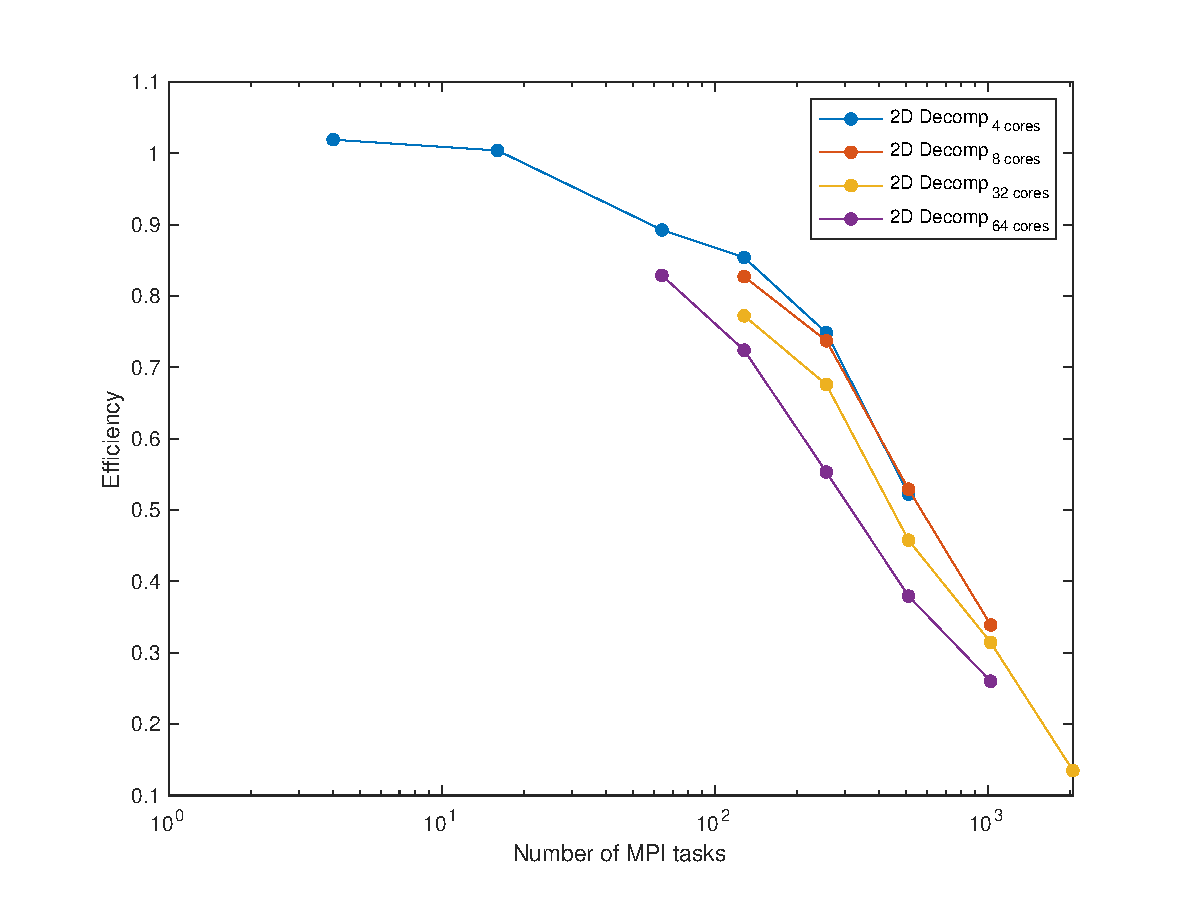
\includegraphics[scale=0.55]{grafici/intel_efficiency}
\caption{Efficiency using 2D decomposition for $256\times 256\times 512$  simulation with Intel Compiler 18}
\label{intel:efficiency}
\end{center}
\end{figure}

As before, the performance peak remains at 1024 simultaneous tasks, however the maximum speedup moved from 178.9, of the 8 cores run using GCC, to 347.1, using the same number of cores with Intel compiler compiled code, with an efficiency not far from the 40\% threshold.
The efficiency gap between the 64 cores runs and the 4 cores ones remains around the 10\%, but the double efficiency with respect to the GCC solution enables the possibility to use 64 cores during production.\\~\\

Next to the already cited flags we used others to refine the auto-vectorization process, in particular the distribution of the MPI tasks among the tiles of the processors, that in this configuration tends to fill adjacent cores with adjacent arrays values, the prefetching level and the mapping of the High Bandwidth Memory, that in this configuration is available as L3 cache memory.
We also moved to a deeper level of optimization and we have disabled fractions in favor to reciprocal multiplications.





\subsection{Performances on GALILeO}


\section{Benchmarks conclusions}
The benchmark series has highlighted common trends present in our simulations.
\par
By looking at the curves, we can see that the performances envelope is bordered by the 64 cores run and the single core ones.  We can catch from the graphs that the code tends to perform faster using as less threads per processor as possible.  This behavior is reasonable, since our code and the library in which we rely on to perform the MPI transposition, does not implement the OpenMP technology at the moment, so, although we could carry on the simulation basing our communications on MPI, we will experience efficiency lacks when dealing with intra-node messagings. In particular, when dealing with many cores per processor we face a speedup tendency to pass from 2 to $2^{2/3}$, as the number of MPI tasks gets doubled, as highlighted in~\cite{dns:gpu:supercomputer}. \par
Unfortunately, the Intel KNL's architecture~\cite{intel:xeonphi} is designed to exploit code vectorization as much as possible and OpenMP plays a key role in this kind of implementations. \par
We suggest to move to traditional processors architectures, instead of using MIC, to experience lower losses. Our simulations in fact has highlighted that, although MPI can not guarantee high efficiency in heavily threaded applications, the lacks using 16 cores, or less, per processor can be acceptable.\\
\par
As the problem size grows, the optimal number of MPI tasks, to achieve the best speedup, grows. In fact, we passed from 512 parallel processes for a $128^{3}$ simulation to 2048 for a $512\times 512 \times1024$ simulation. \par

On the other hand, the speedup factor increase its peak in a fashion which lies on $N\log(N)$ curve, like testify by figure~\ref{speedup:trend} in which our samples are plotted against such behavior. \\
\begin{figure}[h]
\begin{center}
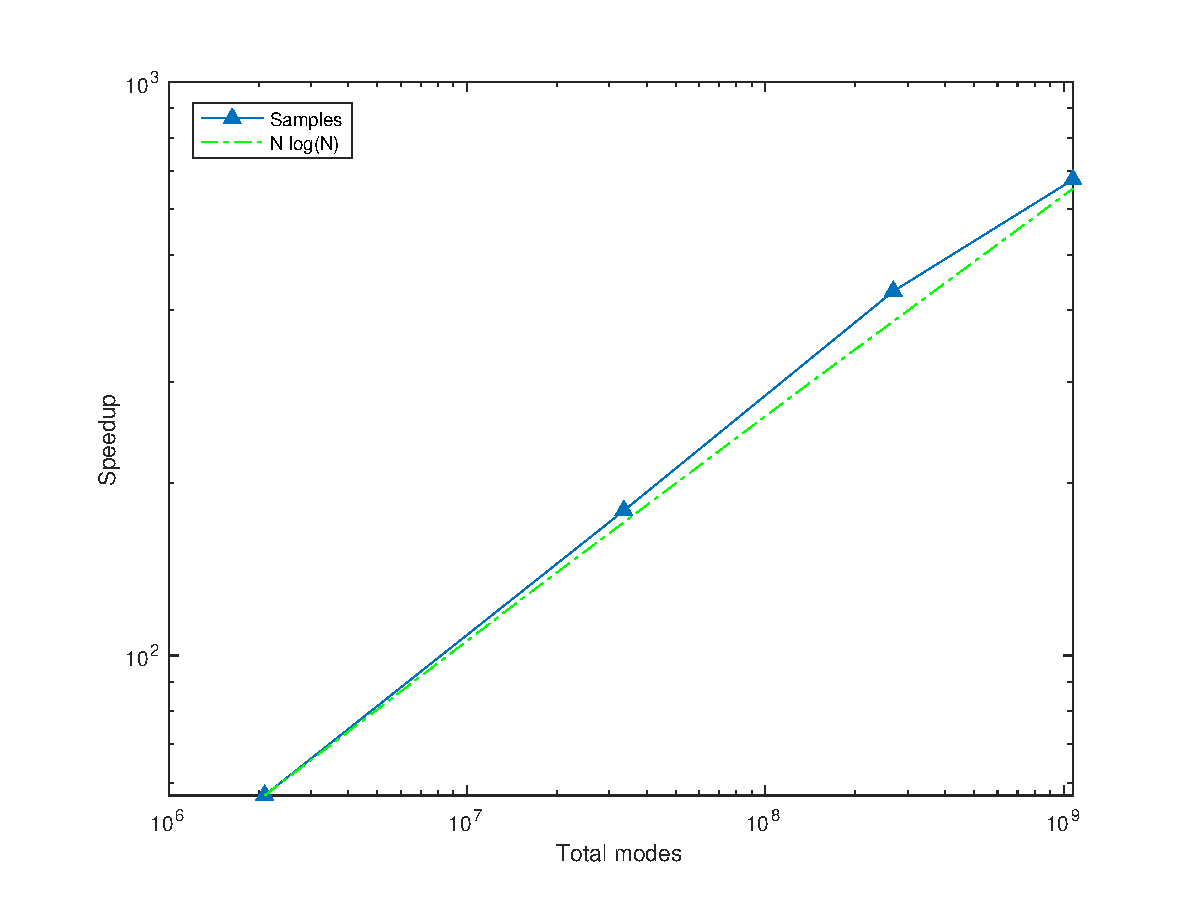
\includegraphics[scale=0.55]{grafici/speedup_trend}
\caption{Speedup factors growth}
\label{speedup:trend}
\end{center}
\end{figure}
\par

Let us introduce the speedup comparison with hyper threading turned on. \par
Hyper threading is a technology developed by Intel~\cite{hyper:paper}  that virtually doubles the cores on the CPU, making the CPU run faster and more efficient by scheduling the workload between the cores. On modern Xeon Phi we can quadruplicate the number of cores, obtaining until 272 threads per processor. However, as our benchmark shows, this technology does not provide a boost in terms of speedup, on the contrary it penalizes our results in evident fashion.\par
In figure~\ref{hyper} are compared the original results of a $512\times 512\times 1024$ simulation, running on different cores per processor, against two curves which exploit the hyper threading technology.\\
\par
In conclusion we would like to show the cost for a single degree of freedom (DOF) in terms of CPU time.
Such cost has been obtained considering the simulation time, the number of time steps required by the simulation and the total number of degrees of freedom, so it has to be intended as a mean value.
The cost is defined as:
\begin{equation}
Time/DOF = \frac{Sim Time}{timestep}\times \frac{1}{nx\times ny\times nz} \times {tasks}
\end{equation}
Our results have been compared with the ones achieved in~\cite{Borrel}, where a boundary layer simulation is carried out on a flat plate, through direct numerical simulation, on JUGENE, a Blue Gene P architecture~\cite{blue:gene:chip}\cite{blue:gene:network} installed at Juelich Forschungszentrum, with its 32,768 cores.\par
Since the problems compared are just similar we can only obtain qualitative informations from that. However, the results of figure~\ref{time:dof} shows good fittings among the data.

\begin{figure}
\begin{center}
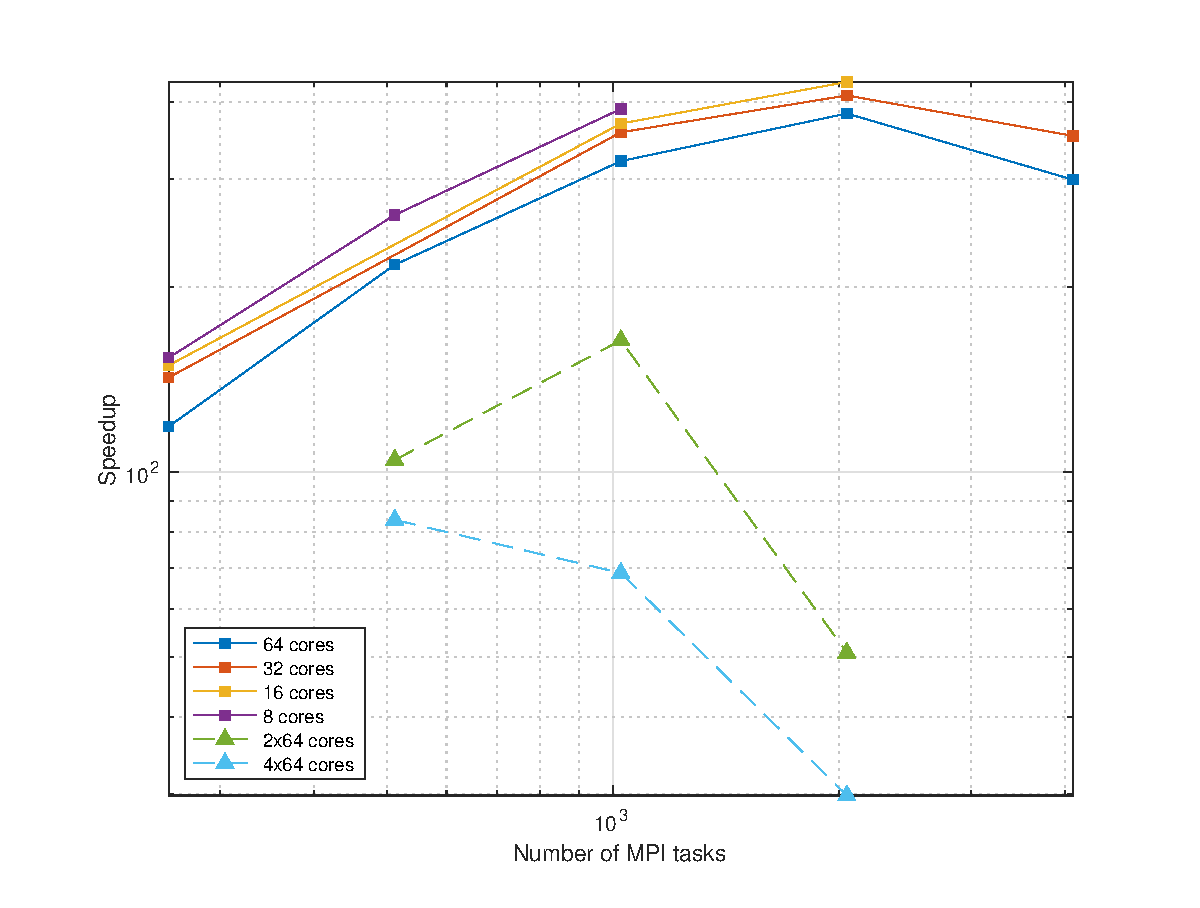
\includegraphics[scale=0.55]{grafici/hyperthreading}
\caption{Hyper threading benchmark}
\label{hyper}
\end{center}
\end{figure}

\begin{figure}
\begin{center}
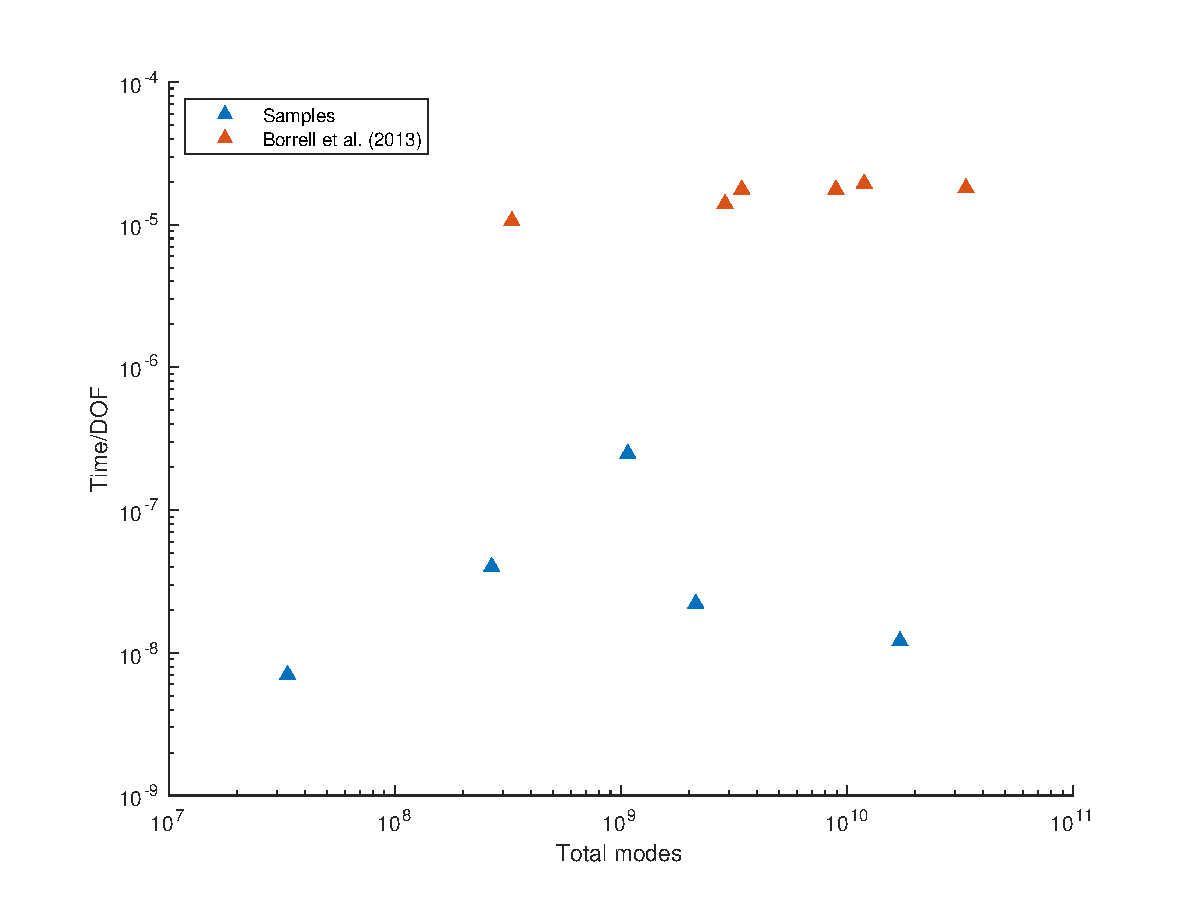
\includegraphics[scale=0.55]{grafici/time_dof}
\caption{Qualitative comparison of Time-DOF ratio}
\label{time:dof}
\end{center}
\end{figure}
